\documentclass[12pt]{article}   	

% Document Formatting Packages
\usepackage{geometry}            		
\geometry{letterpaper}  
\usepackage[usenames,dvipsnames,svgnames,table]{xcolor}


% Document Navigation Packages
\usepackage[parfill]{parskip}          
\usepackage{enumitem}         

% Math Typesetting Tools
\usepackage{amssymb}
\usepackage{amsmath,mathtools}
\usepackage{framed}

% Hyperref
\usepackage[colorlinks=true,linkcolor=blue,citecolor=red]{hyperref}

% Chemistry Typesetting Tools
\usepackage{mhchem}

% Inserting Figures
\usepackage{graphicx}
\usepackage[section]{placeins}
\graphicspath{ {images/} }	
\usepackage[caption=false]{subfig}		

% Miscellaneous Symbol Packages
\usepackage{textcomp}  		
\usepackage{siunitx}
\usepackage{gensymb}

% Set Document Dimensions
\oddsidemargin = 0in
\topmargin = 0in
\headheight=0pt
\headsep = 0pt
\textheight = 9in
\textwidth = 6.5in
\marginparsep = 0in
\marginparwidth = 0in
\footskip = 18pt
\parindent=15pt
\parskip=0pt

% Title
\title{Weekly Update - Week of 06 May 2018}
\author{Joseph Lucero}
\date{\today}

\begin{document}
\maketitle

\section*{Color Coding Guide}

Guide to color coding in these updates:
\begin{itemize}
	\item \textcolor{Red}{Text in red are points that I really want to emphasize and would like your immediate input on as these are either major hurdles that I am currently facing, or important that I get right to ensure that analysis later on is not affected}
	\item \textcolor{ForestGreen}{Text in green are questions that are outstanding that I have not been able to find an answer for, but unlike the text in red these questions these questions are not currently hindering me from progressing forward}
	\item \textcolor{RoyalPurple}{Text in purple are things I just want to stand out apart from my explanations. Thus, things like variable names and major advancements will be colored this way}
\end{itemize}
For your convenience, please feel free to skip most of the text (as it is mostly for me to keep track of progress anyways) but if you could kindly look at what I have highlighted I would greatly appreciate it. Thanks!

\section{Past Week}

This \textbf{past week} I was primarily working on \textbf{two} things:

\begin{enumerate}
	\item \textbf{Start working on creating the geometry for the applicator in Lymperopoulou \textit{et al}. (2004)}
	\begin{itemize}
		\item Used the geometry given in the TG186 applicator folder of egs\_brachy as a template to begin constructing the applicator
		\item Initially ran into some problems regarding the underlying code being unable to successfully run
		\begin{itemize}
			\item Specifically, had problems with the code being unable to create an egsrun folder within my egs\_brachy folder. Got around this by copying the file and adding ``ver2'' at the end of the file name and re-running. This apparently fixed it. (Still not sure what happened here)
			\begin{itemize}
				\item Subsequent renamings of this file did not cause it to crash
			\end{itemize}
			\item Also had some memory problems for a while that turned out to be an error on my part where, because of the order in which I embedded the different geometries, rather than moving the \ce{^{192}Ir} source within the applicator to the different dwell positions, it turns out I was moving the entire applicator.
		\end{itemize}
		\item Finished constructing the geometry of the applicator and have successfully embedded the \ce{^{192}Ir} dwell positions within it.
	\end{itemize}
	\item \textbf{Run initial simulations on prototype geometry}
	\begin{itemize}
		\item I embedded the applicator, centered, into a cubic water phantom with the dimensions of $ \left(20\ \si{\centi\meter}\right)^{3} $ with cubic scoring voxels of size $ \left(2\ \si{\milli\meter}\right)^{3} $.
		\item The water phantom was then surrounded by $ 10\ \si{\centi\meter} $ water padding on each side 
		\item Total simulation geometry was a cube with dimensions $ \left(30\ \si{\centi\meter}\right)^{3} $
		\begin{itemize}
			\item \textcolor{Red}{This is roughly in line with Lymperopoulou \textit{et al}. Though there it seems that they had a spherical water phantom but cubic scoring voxels?} (This still doesn't make sense to me. I have to re-read the paper)
			\item I also have not yet figured out how they ``programmed'' the location of the source dwell positions. So I tried a series of different positions to see what effects they would have and which ones most closely matched their results
		\end{itemize}
		\item Because my phantom geometry is much more different than what Lymperopoulou \textit{et al}. have I am getting much more different numbers that what they report in the paper
		\item Below I have attached the results from the simulations I have run thus far
		\item I have run simulations for the configuration described above for an applicator with no shielding, $ 90\degree $ shielding, $ 180\degree $ shielding, $ 270\degree $ shielding and the results and a bit of discussion are below
	\end{itemize}
\end{enumerate}

\section{Next Week}

In the \textbf{next week} I plan on tackling the following \textbf{three} things:

\begin{enumerate}
	\item \textbf{Continue with my readings}
	\begin{itemize}
		\item Read about fundamentals of brachytherapy
		\item Read about the relevant statistics in use clinical dosimetry
		\item Read the paper by Ma \textit{et al}. (2017)
	\end{itemize}
	\item \textbf{Do comparison with Suxer's results and see what is different between our simulation results}
\end{enumerate}	

\section{Figures}

A quick explanation regarding the labels:
\begin{itemize}
	\item Here ``configuration'' means the different possible dwell positions that I have tried (temporary lack of a better name) they are as follows (listing the location of the dwell positions within in units of cm):
	\begin{enumerate}
		\item Base config.: 4.0, 4.5, 5.0, 5.5, 6.0, 6.5, 7.0
		\item Config. 2: 3.5, 4.0, 4.5, 5.0, 5.5, 6.0, 6.5
		\item Config. 3: 3.0, 3.5, 4.0, 4.5, 5.0, 5.5, 6.0
		\item Config. 4: 2.5, 3.0, 3.5, 4.0, 4.5, 5.0, 5.5
		\item Config. 5: 2.0, 2.5, 3.0, 3.5, 4.0, 4.5, 5.0
		\item Config. 6: 1.5, 2.0, 2.5, 3.0, 3.5, 4.0, 4.5
		\item Config. 7: 4.5, 5.0, 5.5, 6.0, 6.5, 7.0, 7.5
		\item Config. 8: 5.0, 5.5, 6.0, 6.5, 7.0, 7.5, 8.0
	\end{enumerate}
	\item The midpoint of the \emph{cylindrical} portion of the applicator is the origin.
\end{itemize}

\subsection{No Shield}

\begin{figure}[!ht]
	\centering
	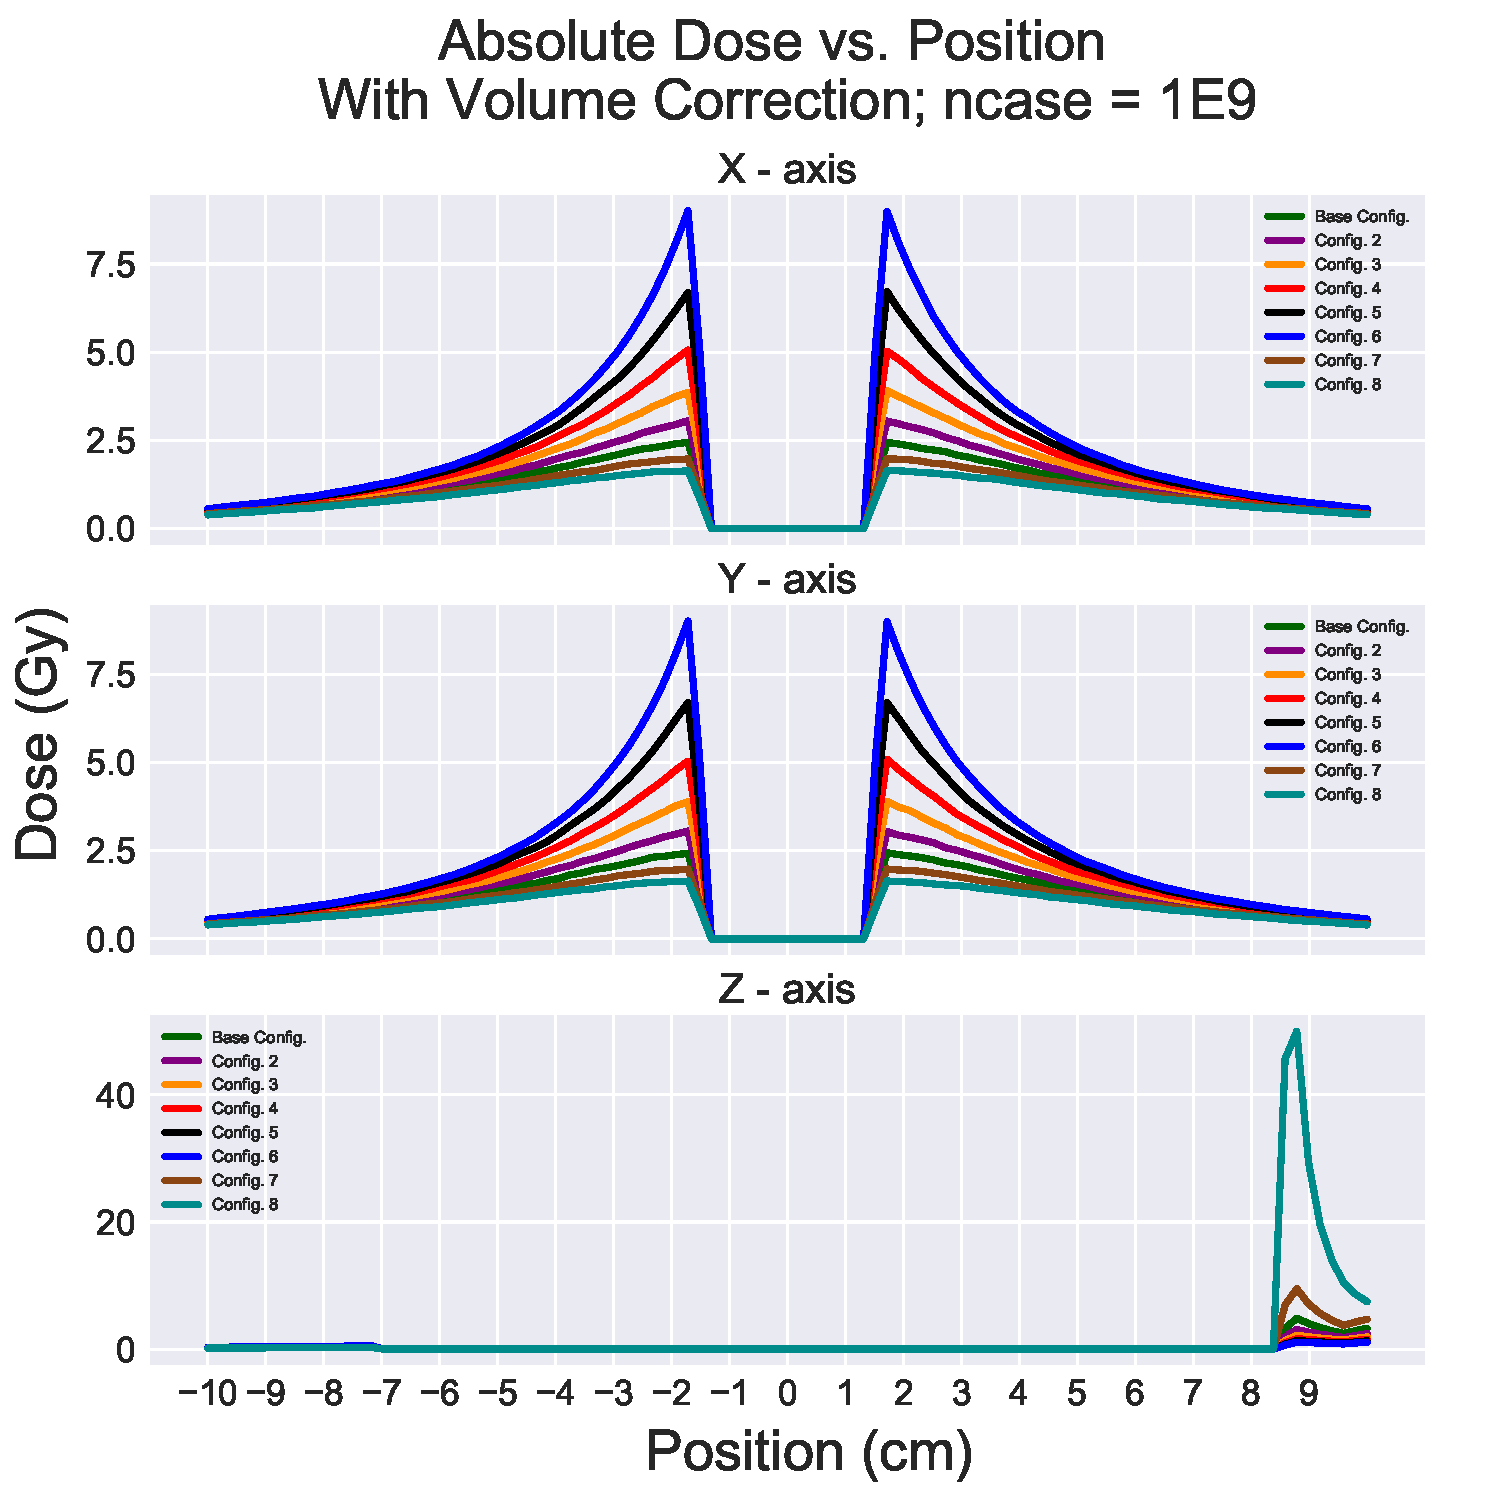
\includegraphics[scale=0.6]{dosage_comparison_noShield}
	\caption{Absolute Dose vs. Position with respect to the coordinate planes.}
\end{figure}

\begin{figure}[!ht]
	\centering
	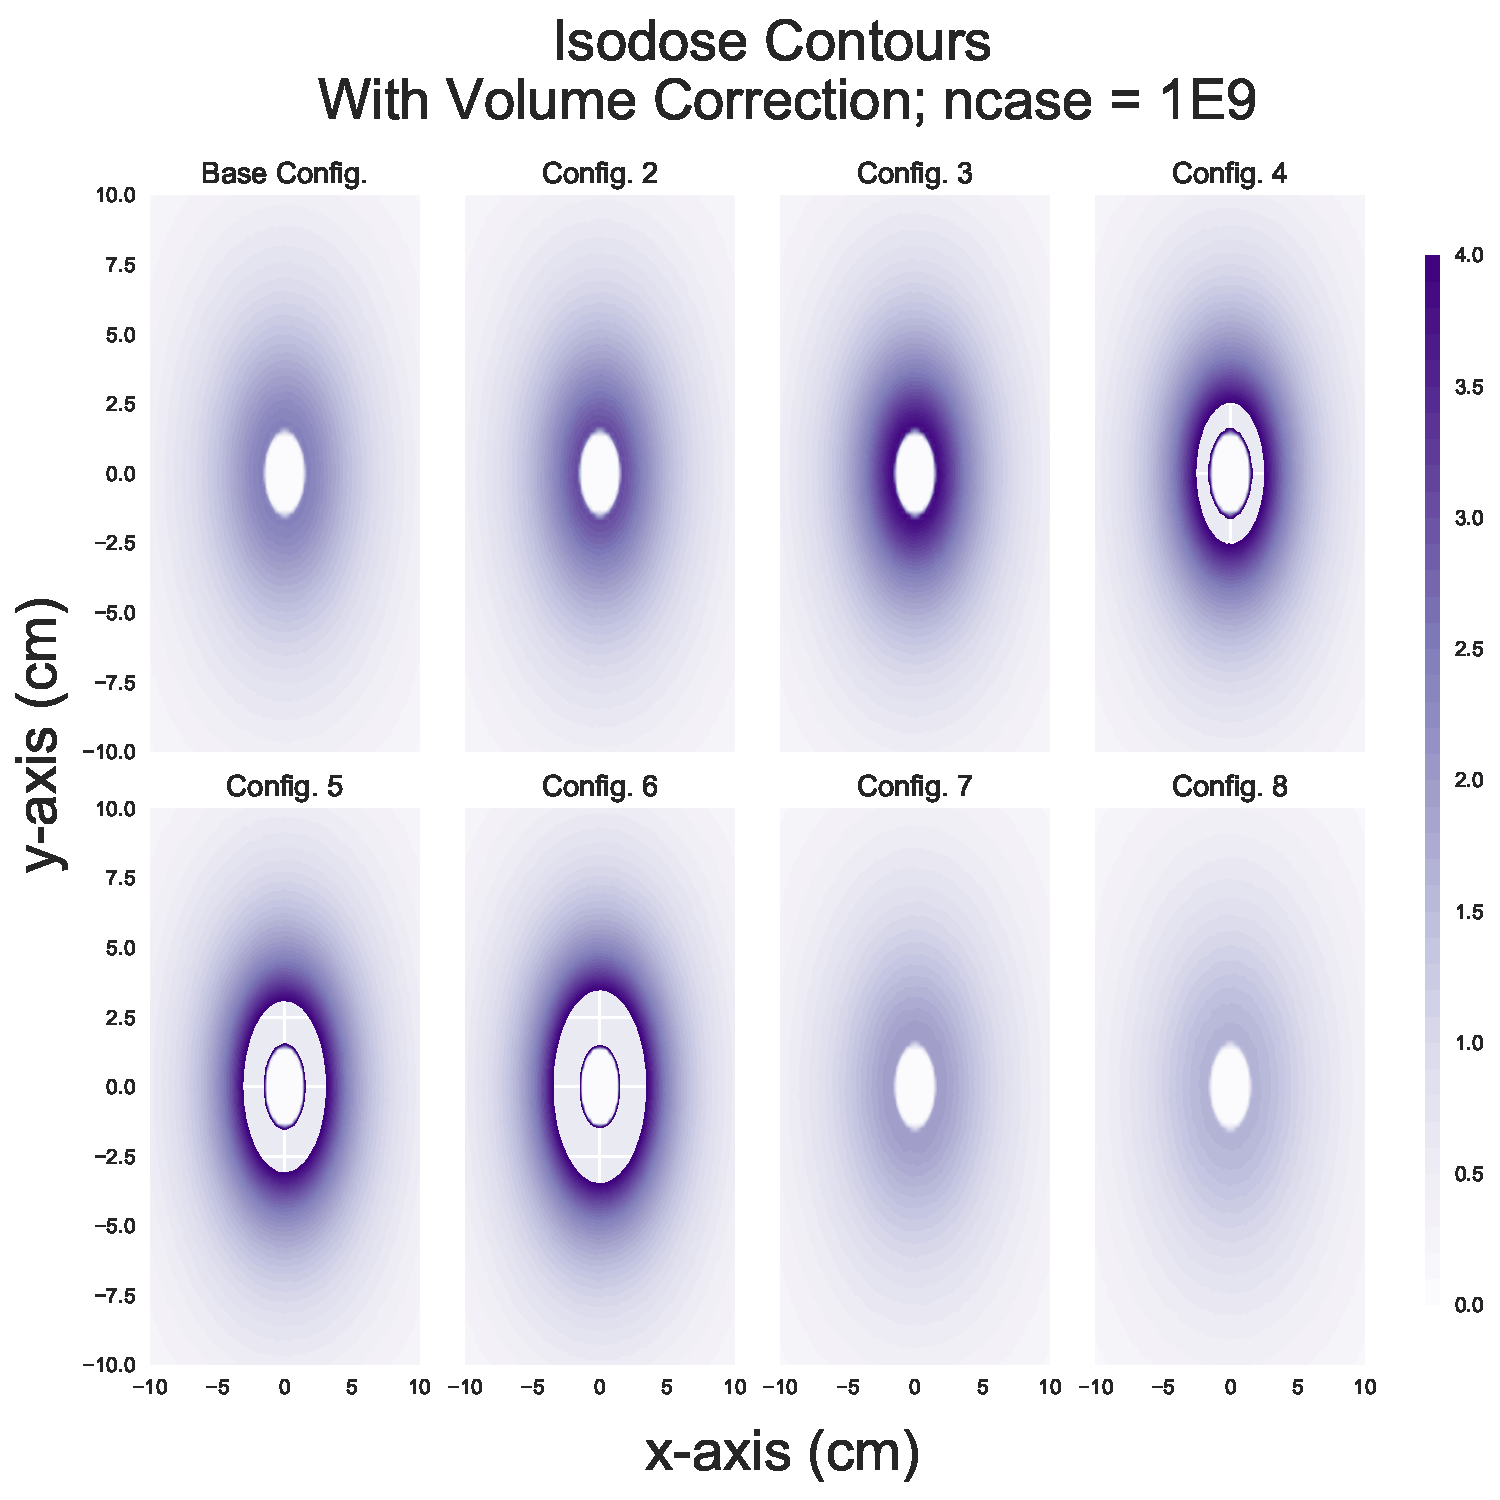
\includegraphics[scale=0.6]{xy_isodose_profiles_noShield}
	\caption{Isodose contours on the xy-plane.}
\end{figure}

\begin{figure}[!ht]
	\centering
	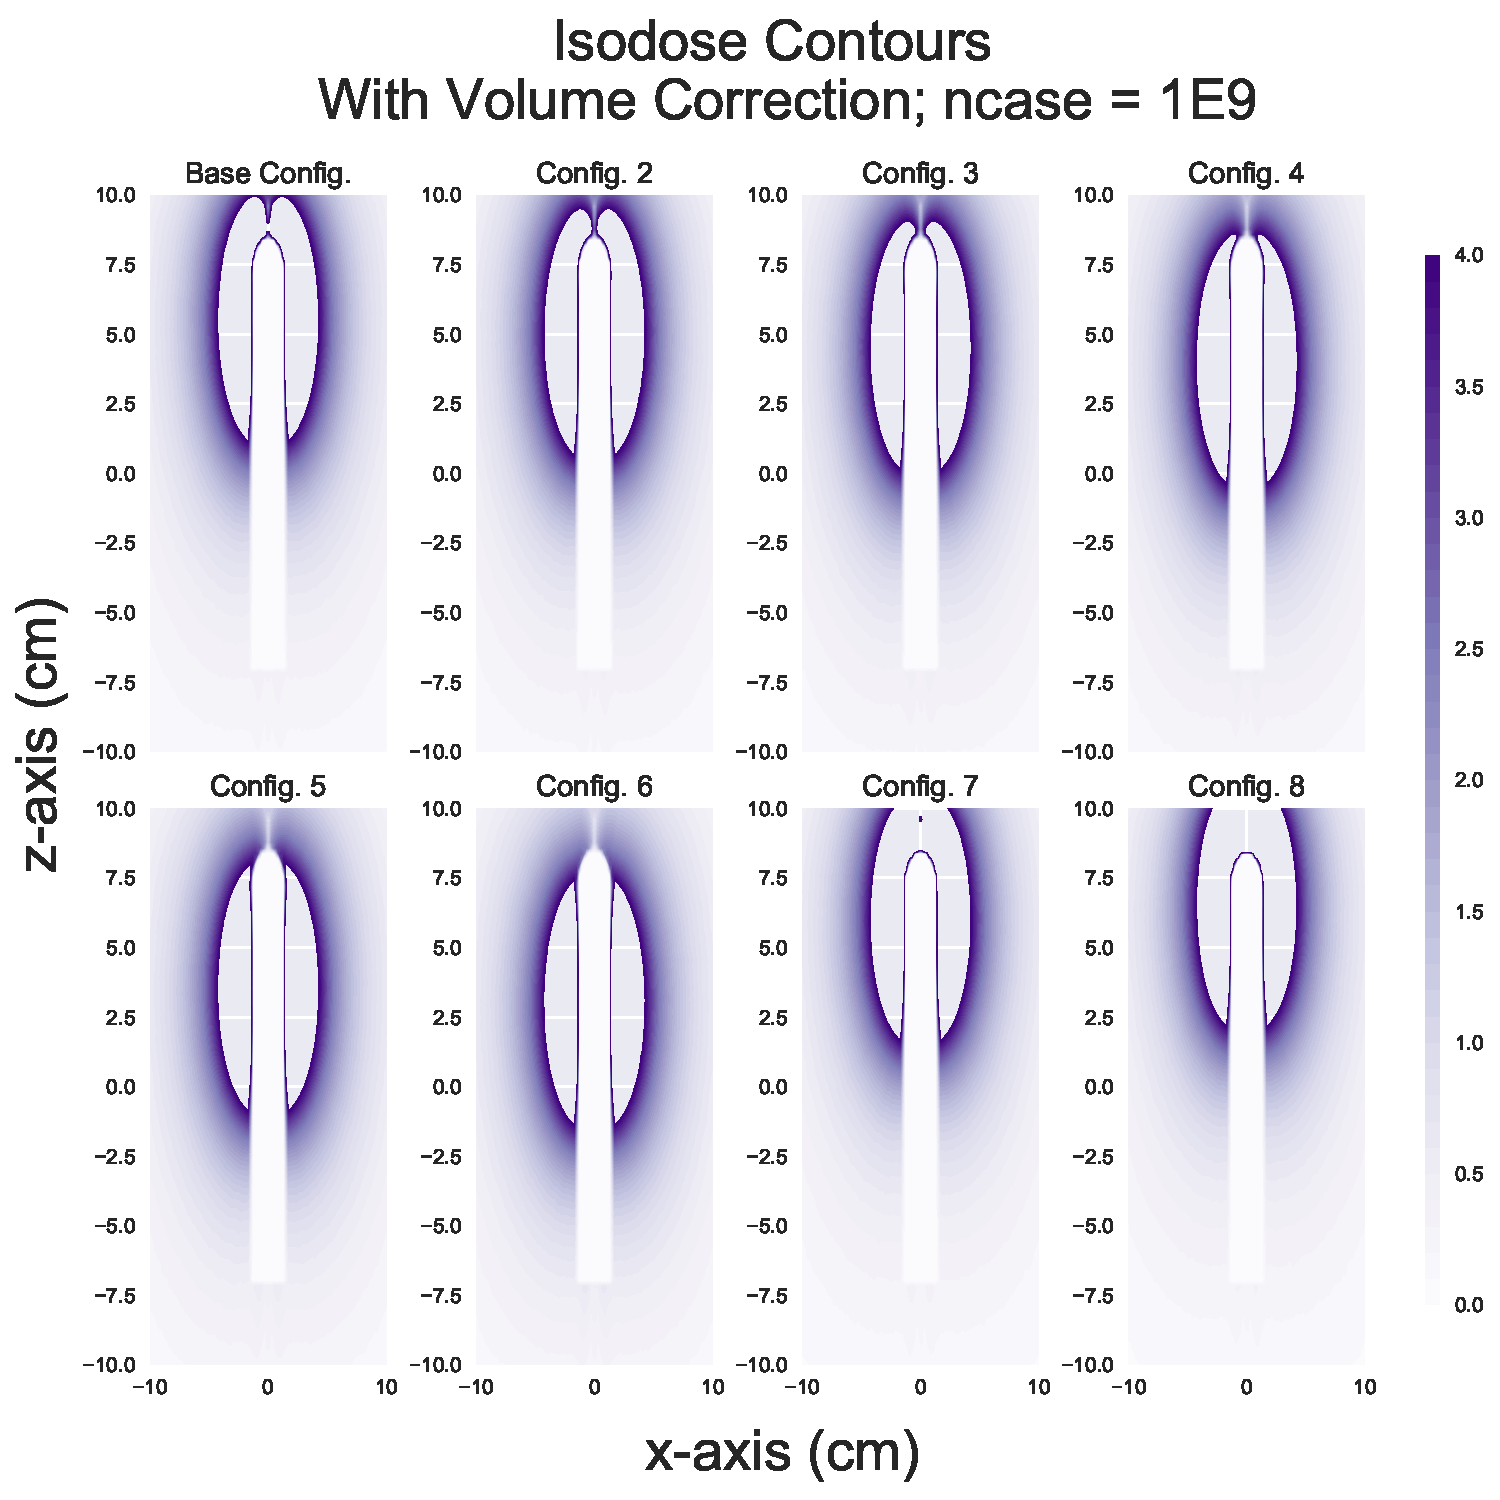
\includegraphics[scale=0.6]{xz_isodose_profiles_noShield}
	\caption{Isodose contours on the xy-plane.}
\end{figure}

\FloatBarrier

\subsection{90$\degree$ shield}

\begin{figure}[!ht]
	\centering
	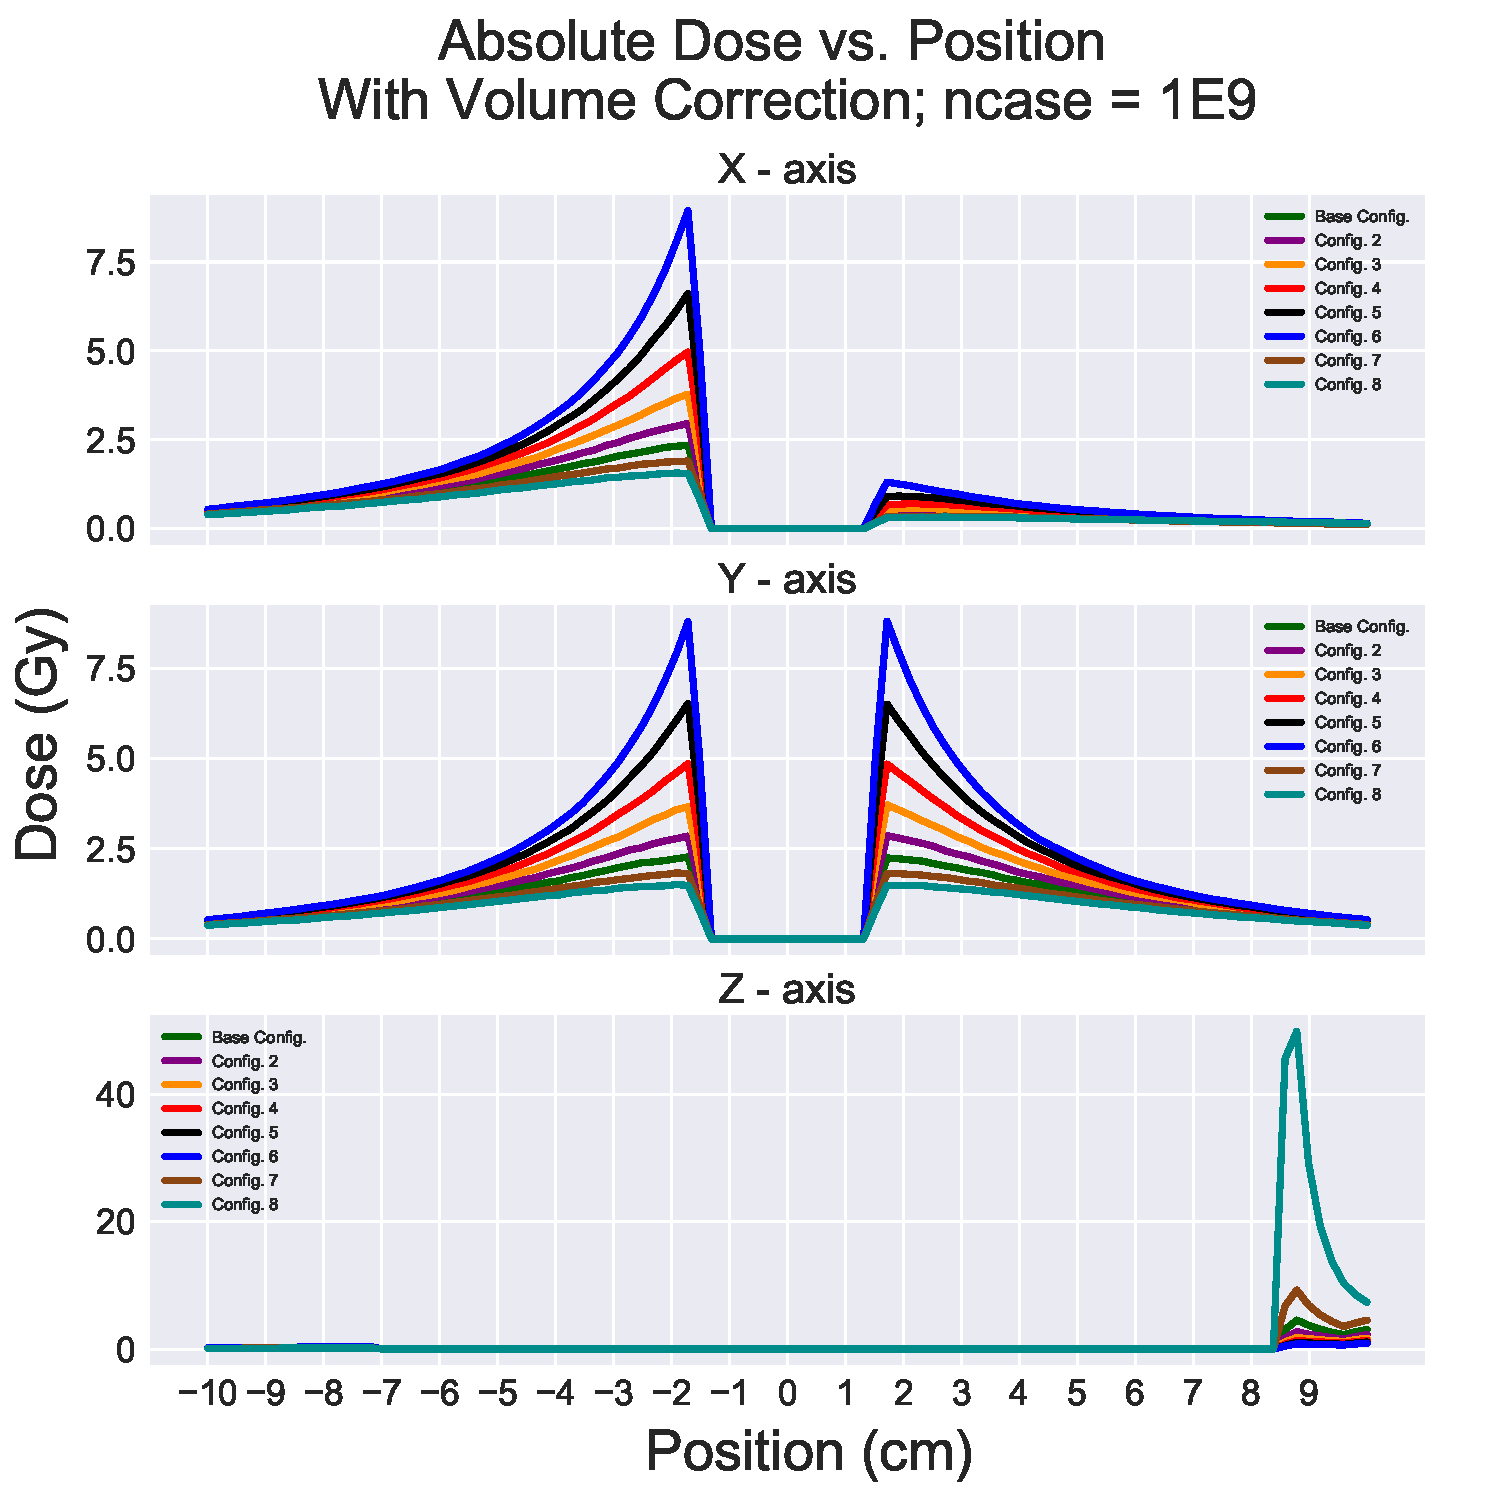
\includegraphics[scale=0.6]{dosage_comparison_90Shield}
	\caption{Absolute Dose vs. Position with respect to the coordinate planes.}
\end{figure}

\begin{figure}[!ht]
	\centering
	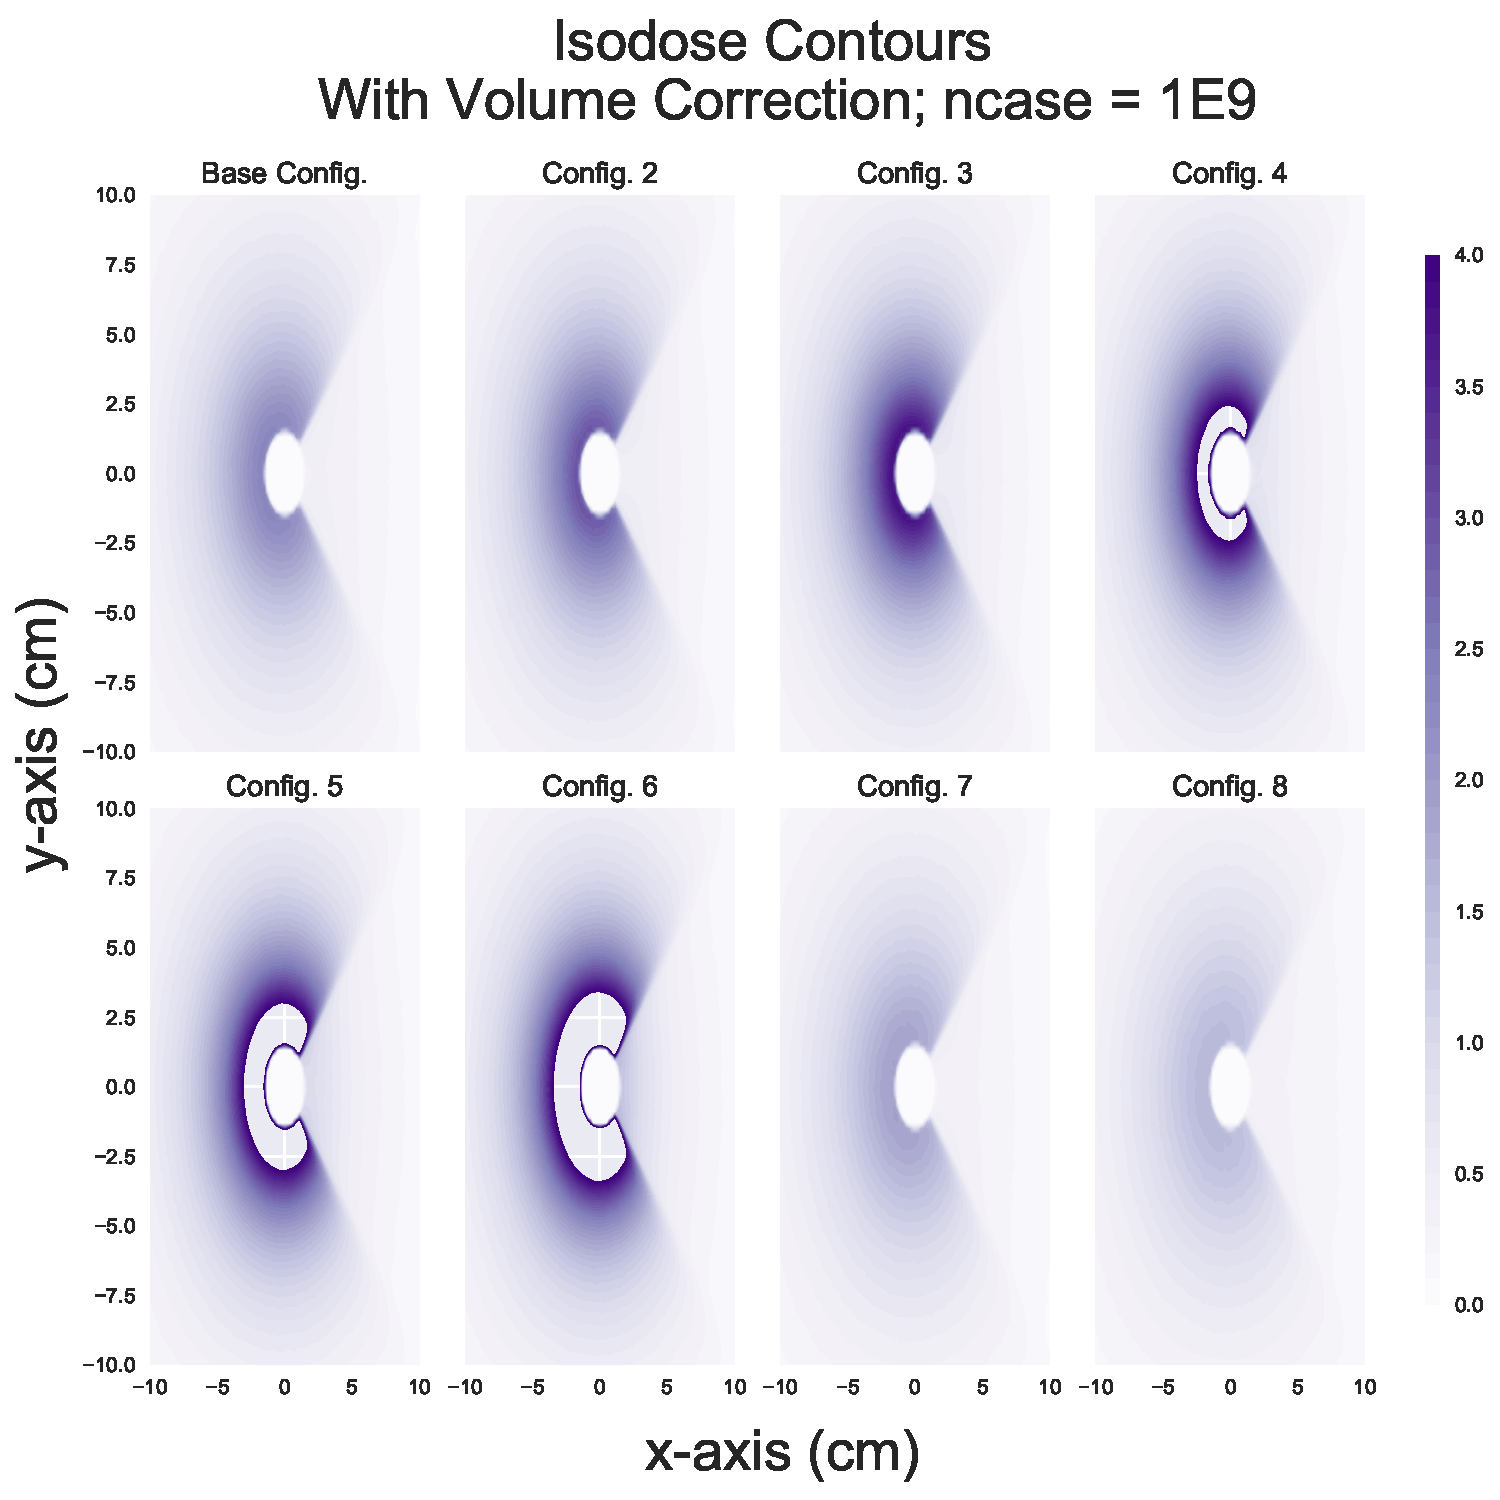
\includegraphics[scale=0.6]{xy_isodose_profiles_90Shield}
	\caption{Isodose contours on the xy-plane.}
\end{figure}

\begin{figure}[!ht]
	\centering
	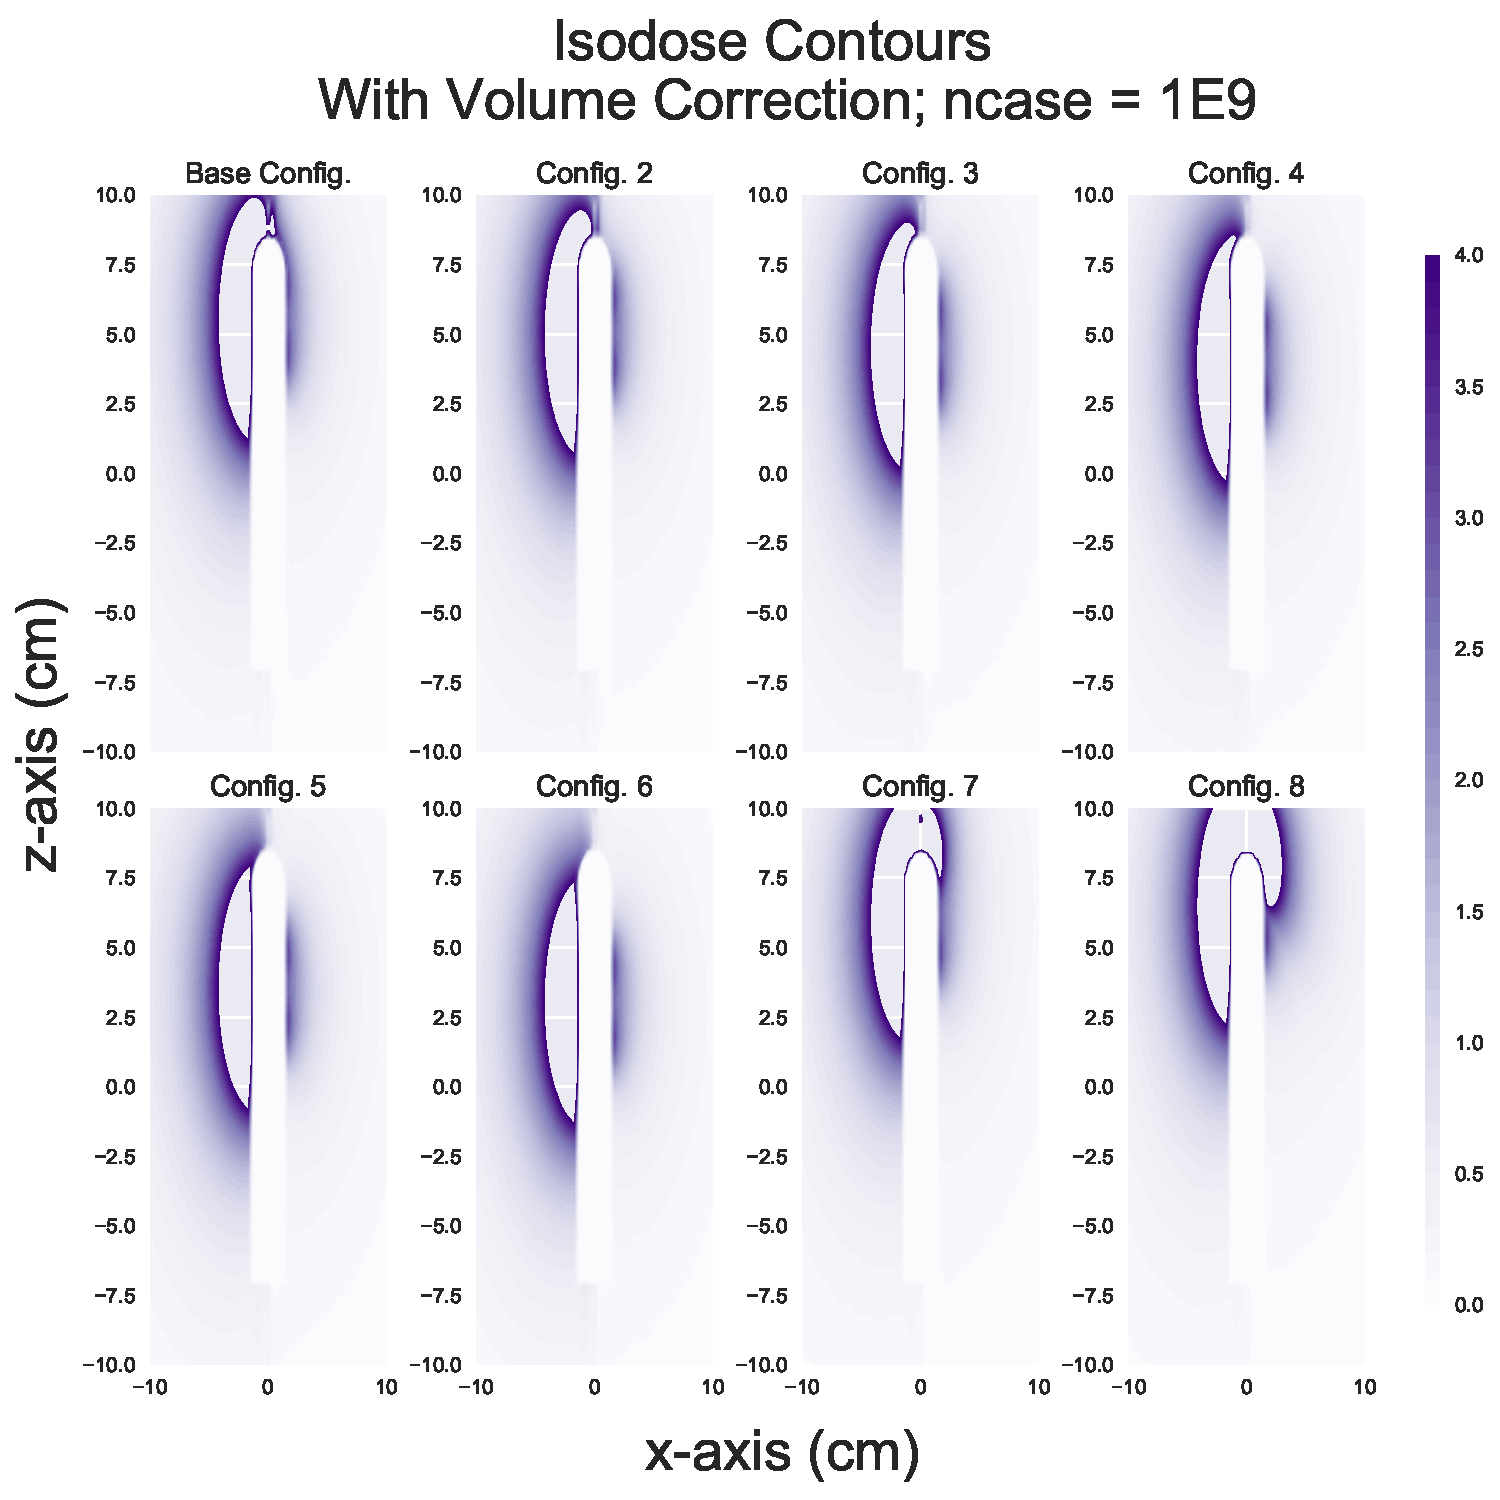
\includegraphics[scale=0.6]{xz_isodose_profiles_90Shield}
	\caption{Isodose contours on the xz-plane.}
\end{figure}

\FloatBarrier

\subsection{180$\degree$ shield}

\begin{figure}[!ht]
	\centering
	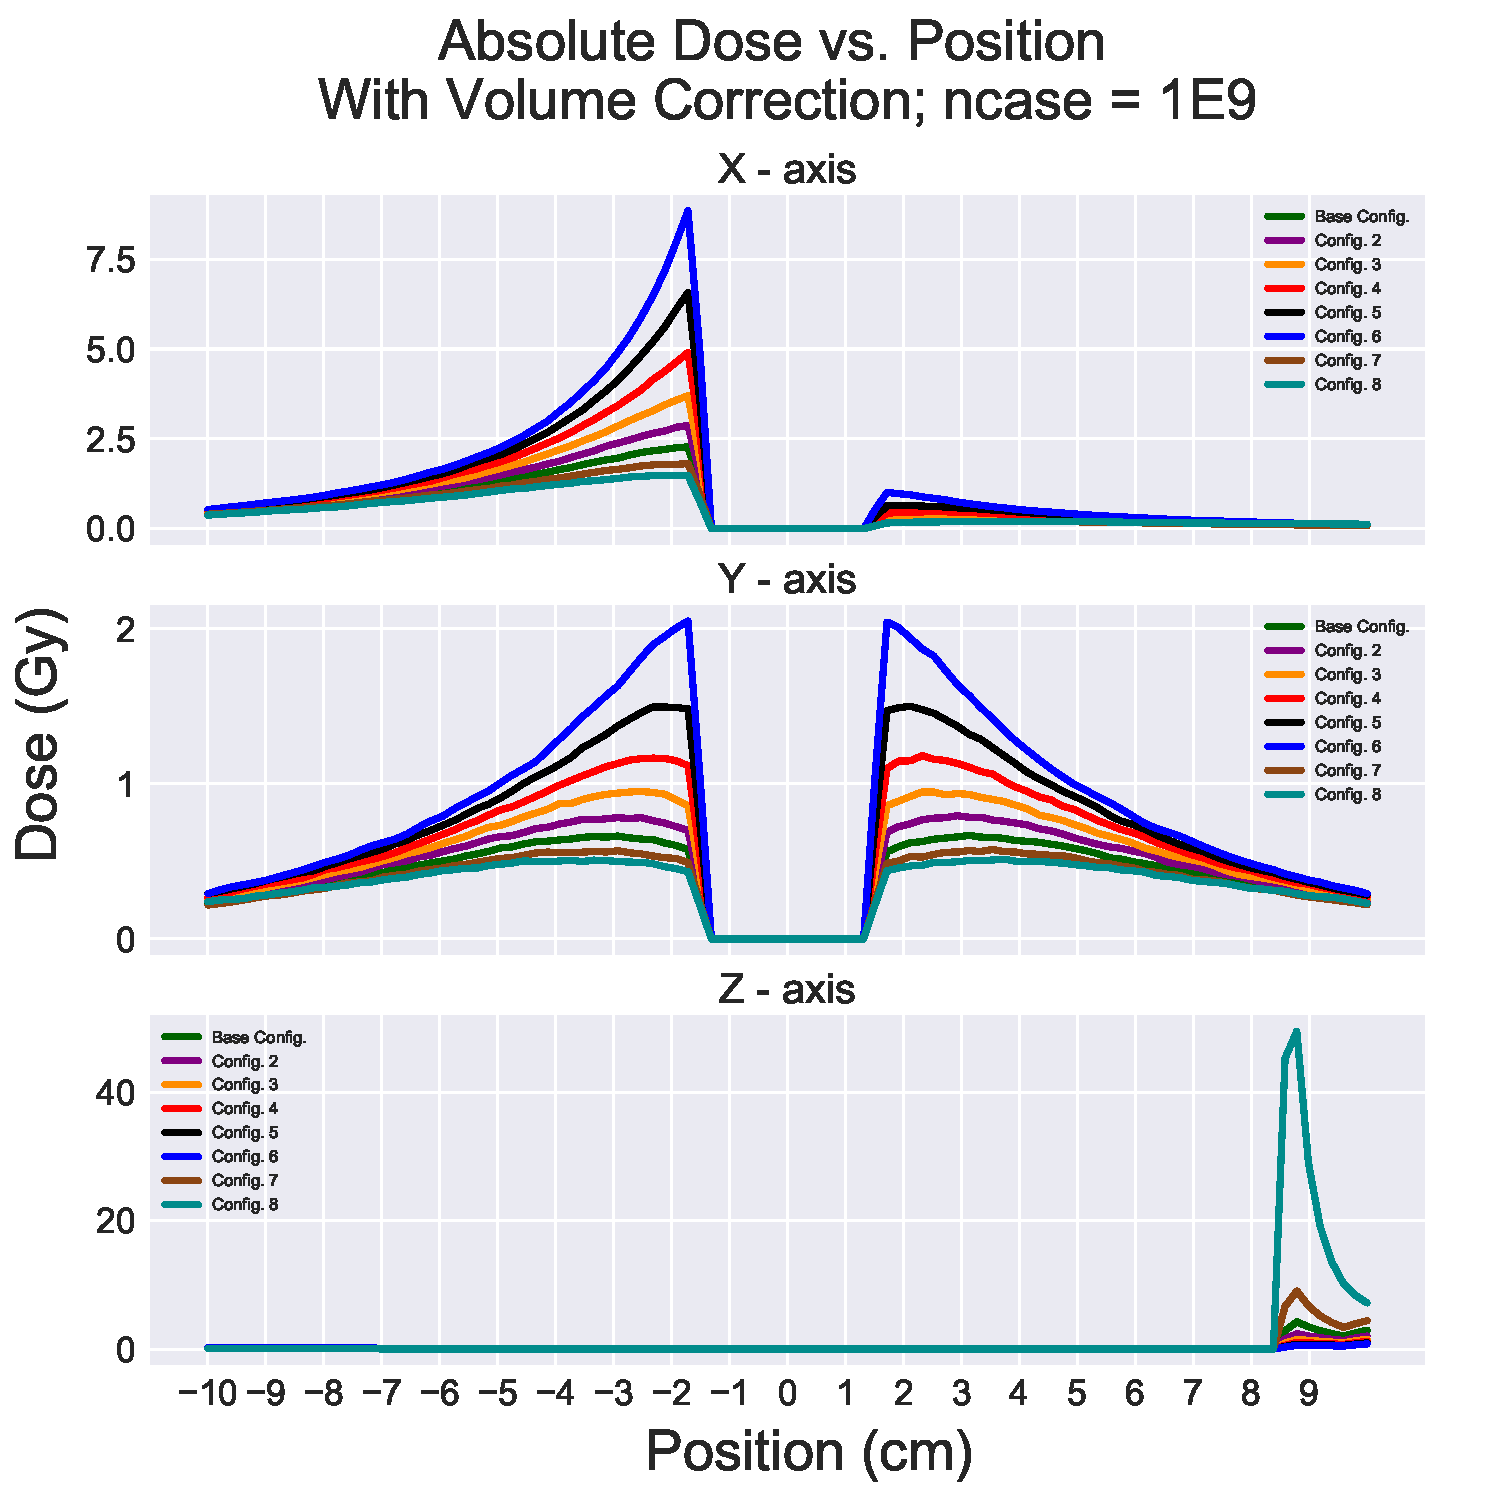
\includegraphics[scale=0.6]{dosage_comparison_180Shield}
	\caption{Absolute Dose vs. Position with respect to the coordinate planes.}
\end{figure}

\begin{figure}[!ht]
	\centering
	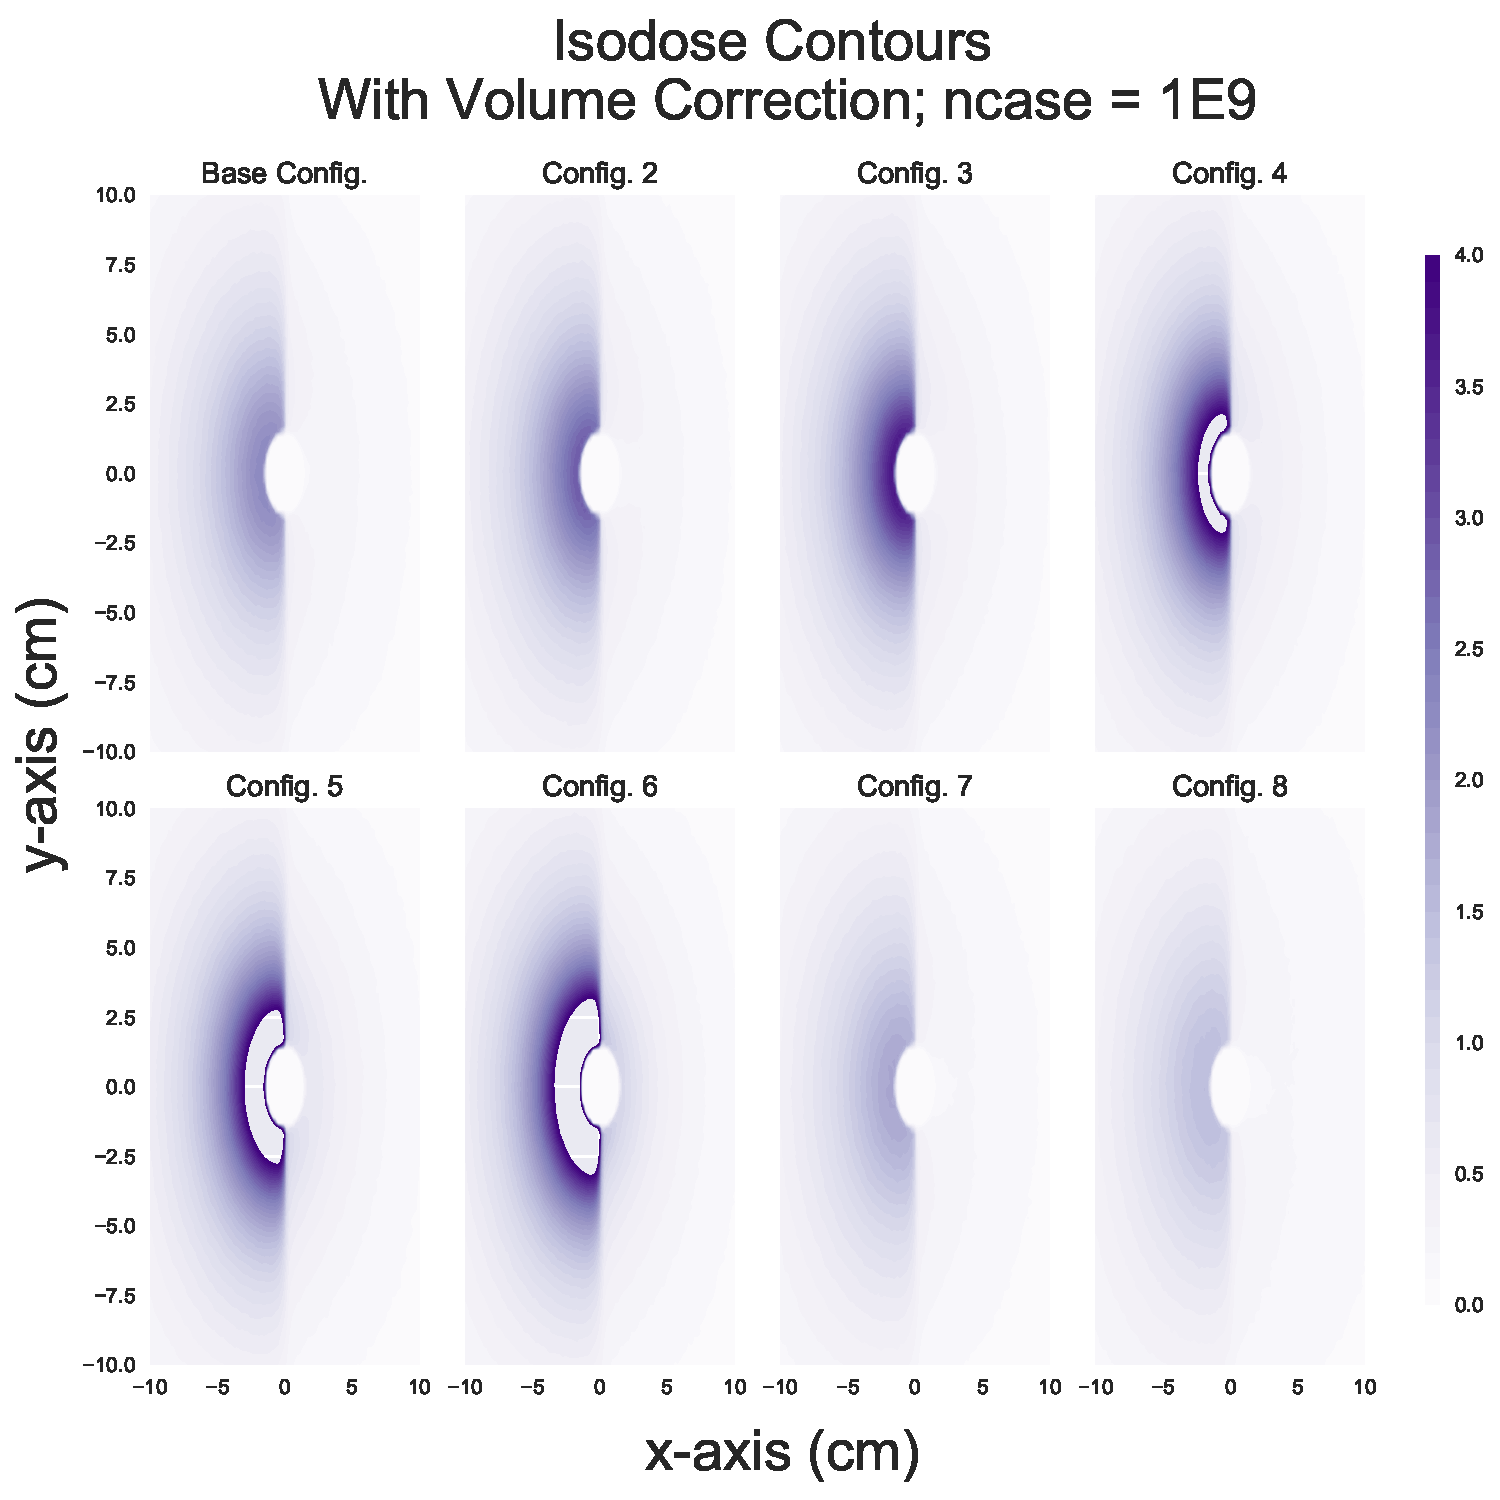
\includegraphics[scale=0.6]{xy_isodose_profiles_180Shield}
	\caption{Isodose contours on the xy-plane.}
\end{figure}

\begin{figure}[!ht]
	\centering
	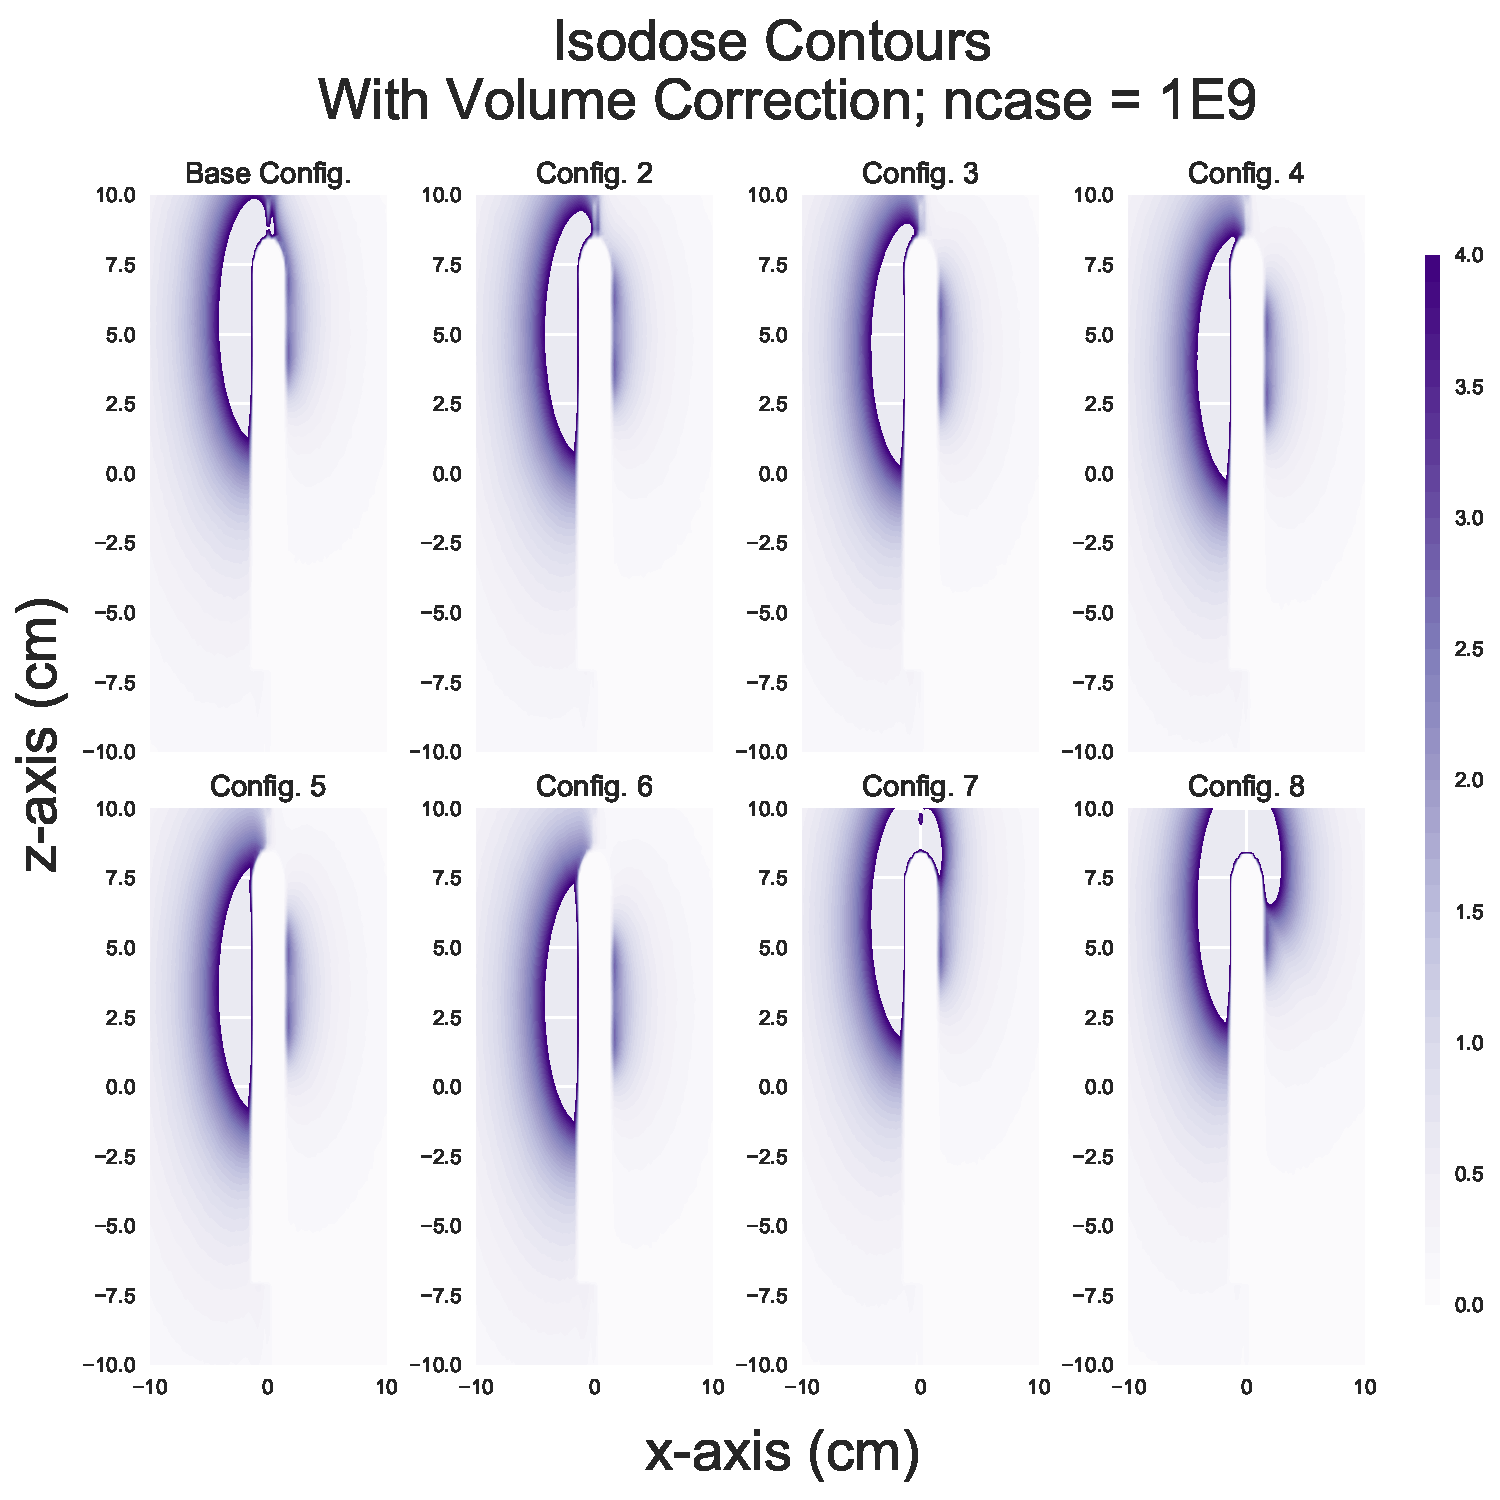
\includegraphics[scale=0.6]{xz_isodose_profiles_180Shield}
	\caption{Isodose contours on the xz-plane.}
\end{figure}

\FloatBarrier

\subsection{270$\degree$ shield}

\begin{figure}[!ht]
	\centering
	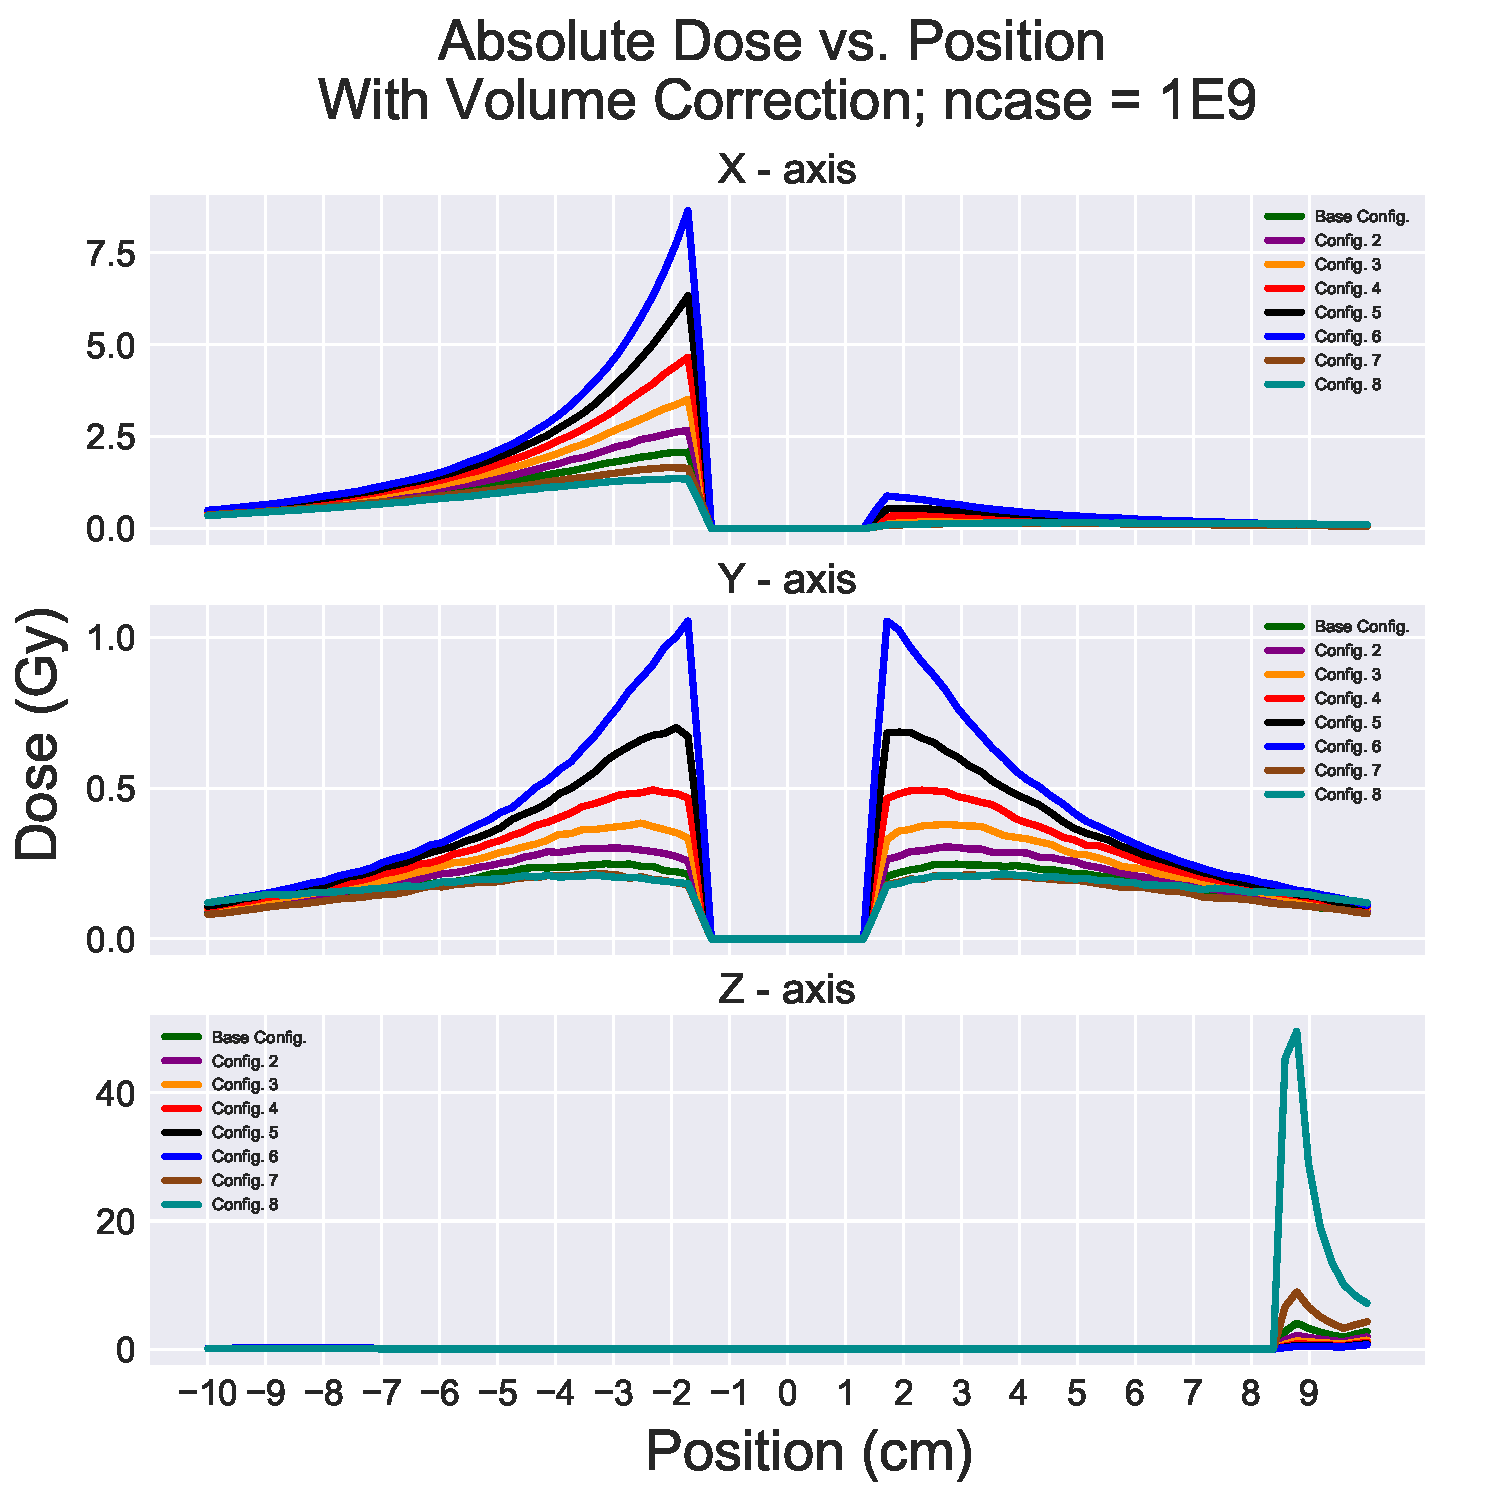
\includegraphics[scale=0.6]{dosage_comparison_270Shield}
	\caption{Absolute Dose vs. Position with respect to the coordinate planes.}
\end{figure}

\begin{figure}[!ht]
	\centering
	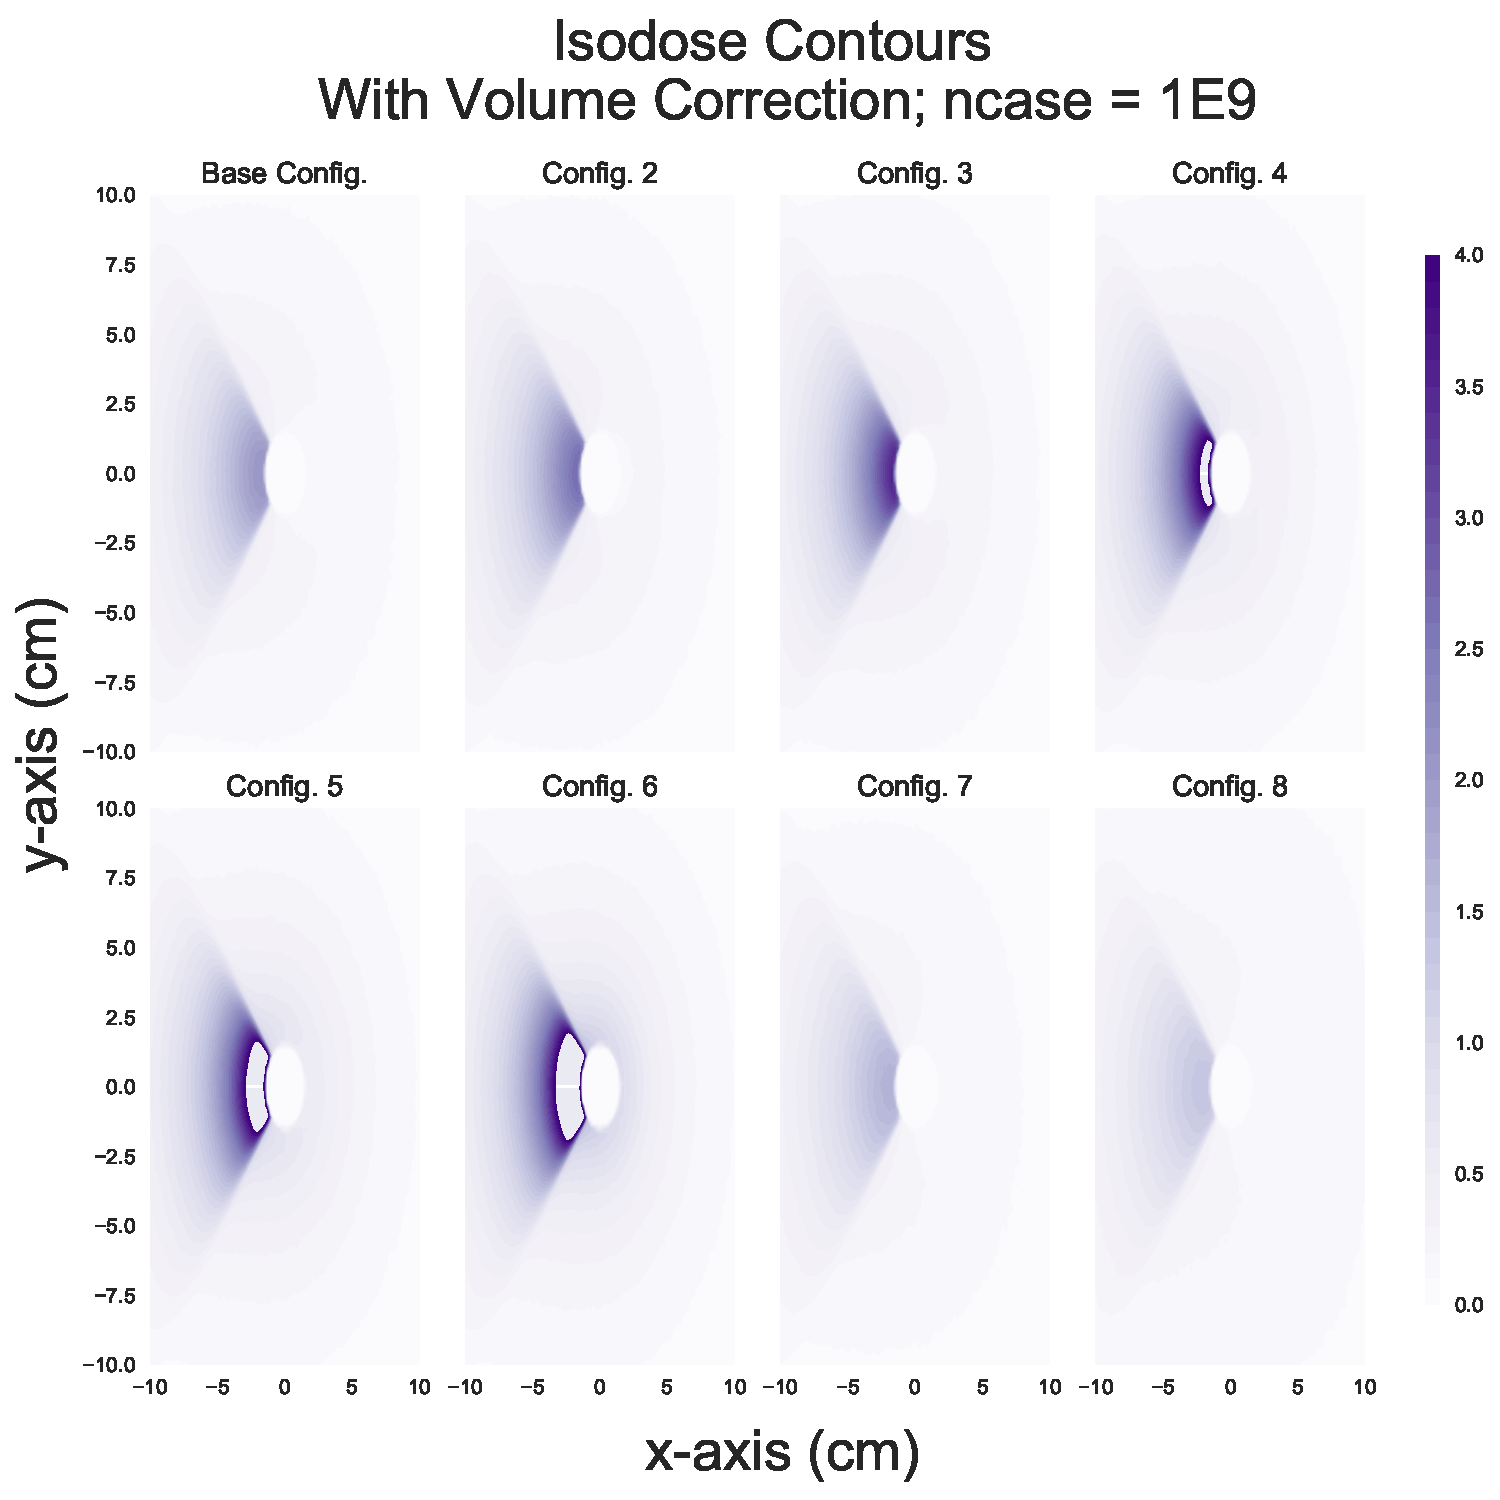
\includegraphics[scale=0.6]{xy_isodose_profiles_270Shield}
	\caption{Isodose contours on the xy-plane.}
\end{figure}

\begin{figure}[!ht]
	\centering
	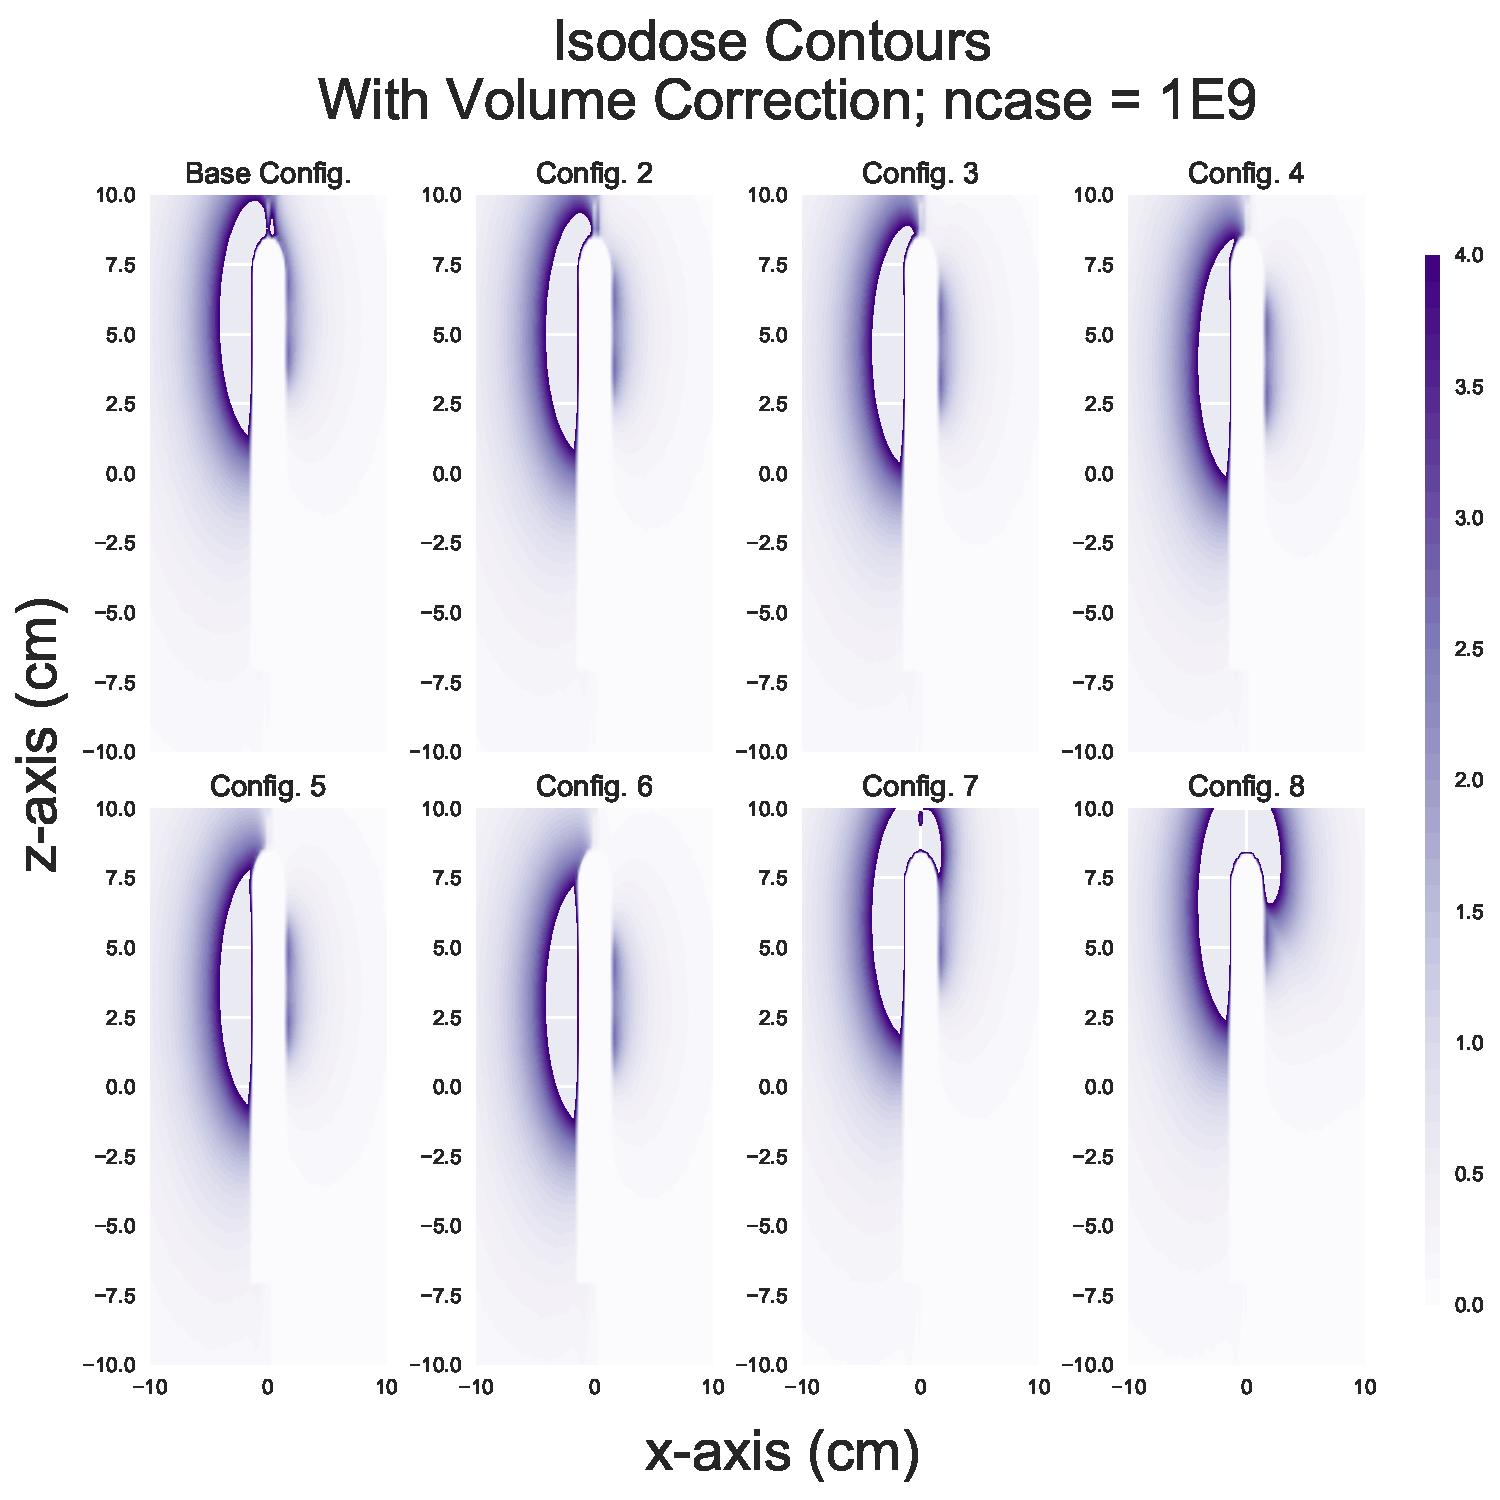
\includegraphics[scale=0.6]{xz_isodose_profiles_270Shield}
	\caption{Isodose contours on the xz-plane.}
\end{figure}

\FloatBarrier

\subsection{Dose Volume Histograms}

\begin{figure}[!ht]
	\centering
	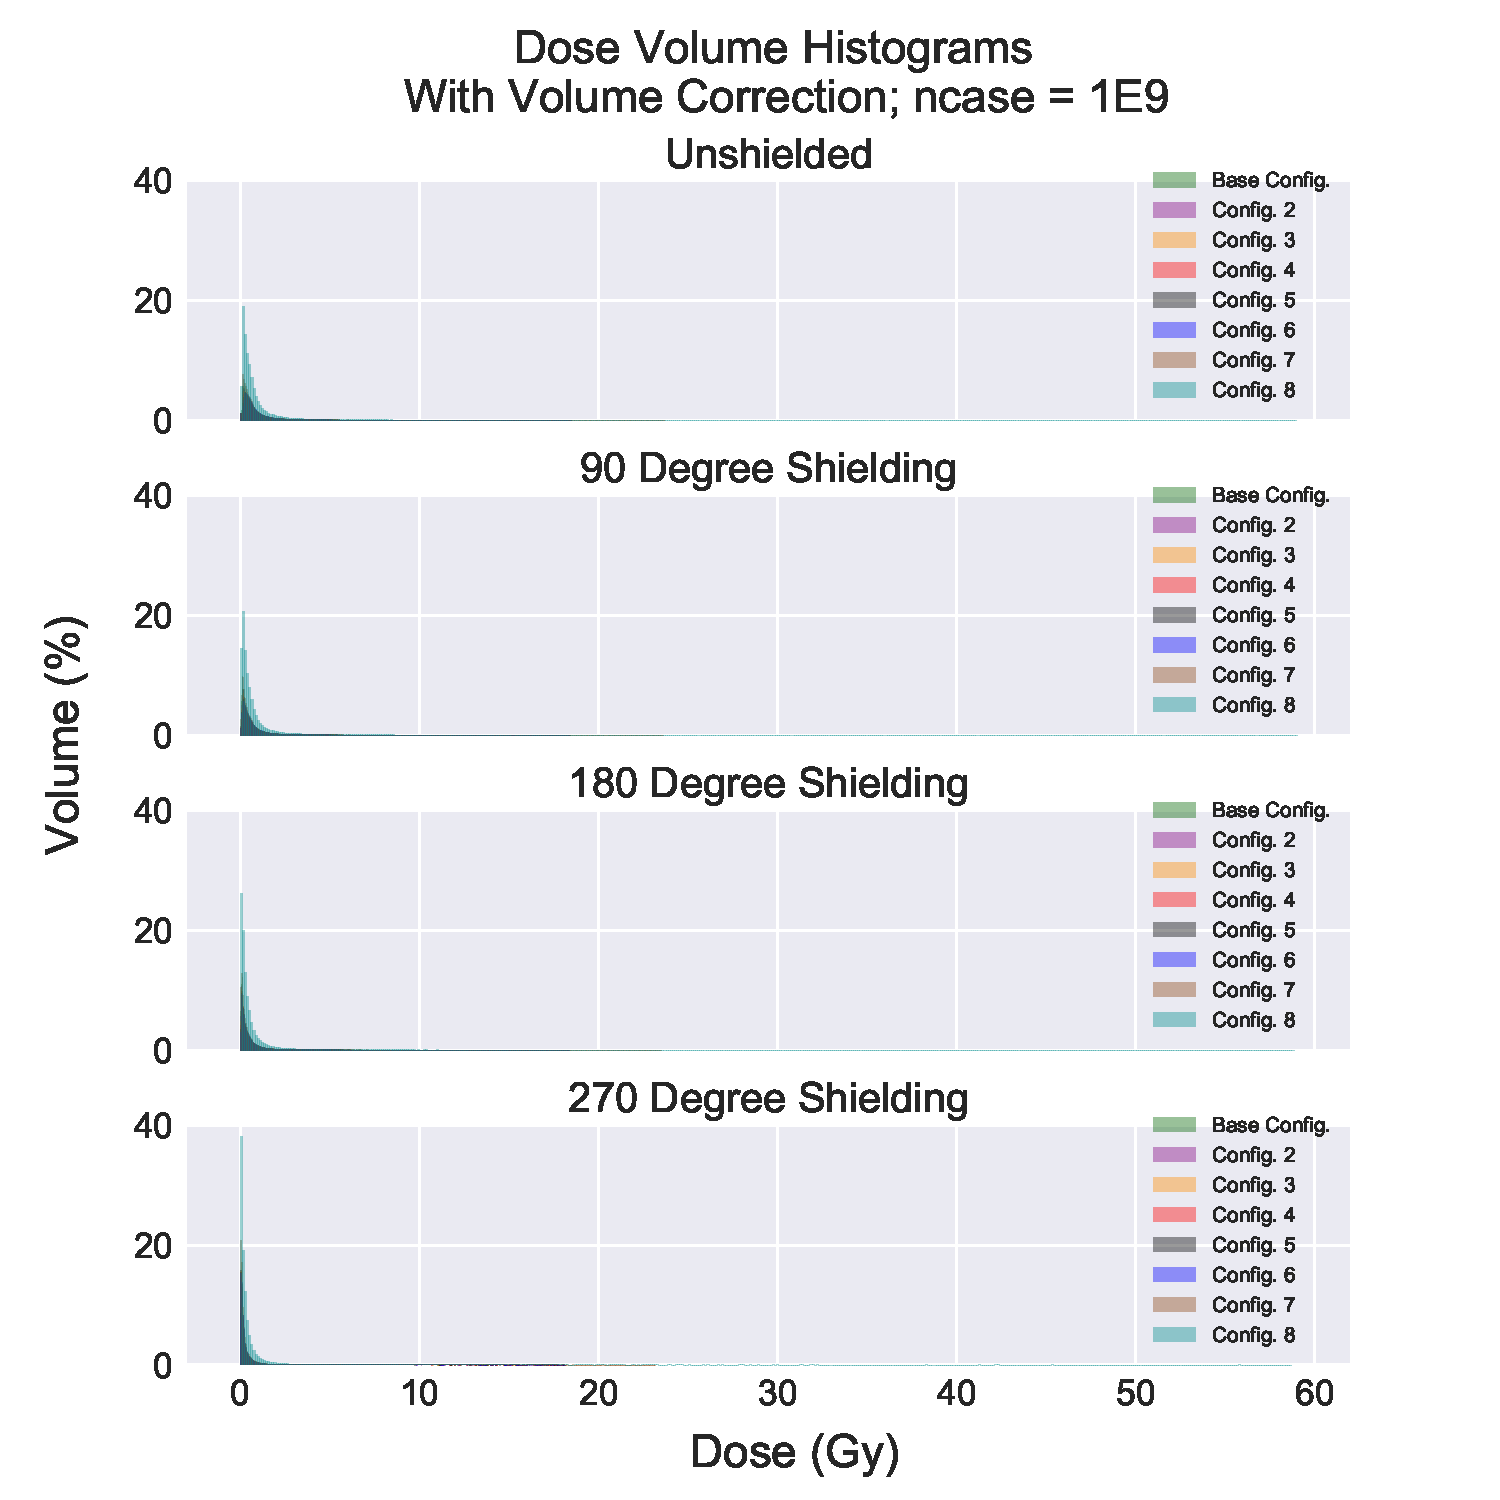
\includegraphics[scale=0.6]{dose_volume_histogram}
	\caption{Absolute Dose Volume Histograms}
\end{figure}

\begin{figure}[!ht]
	\centering
	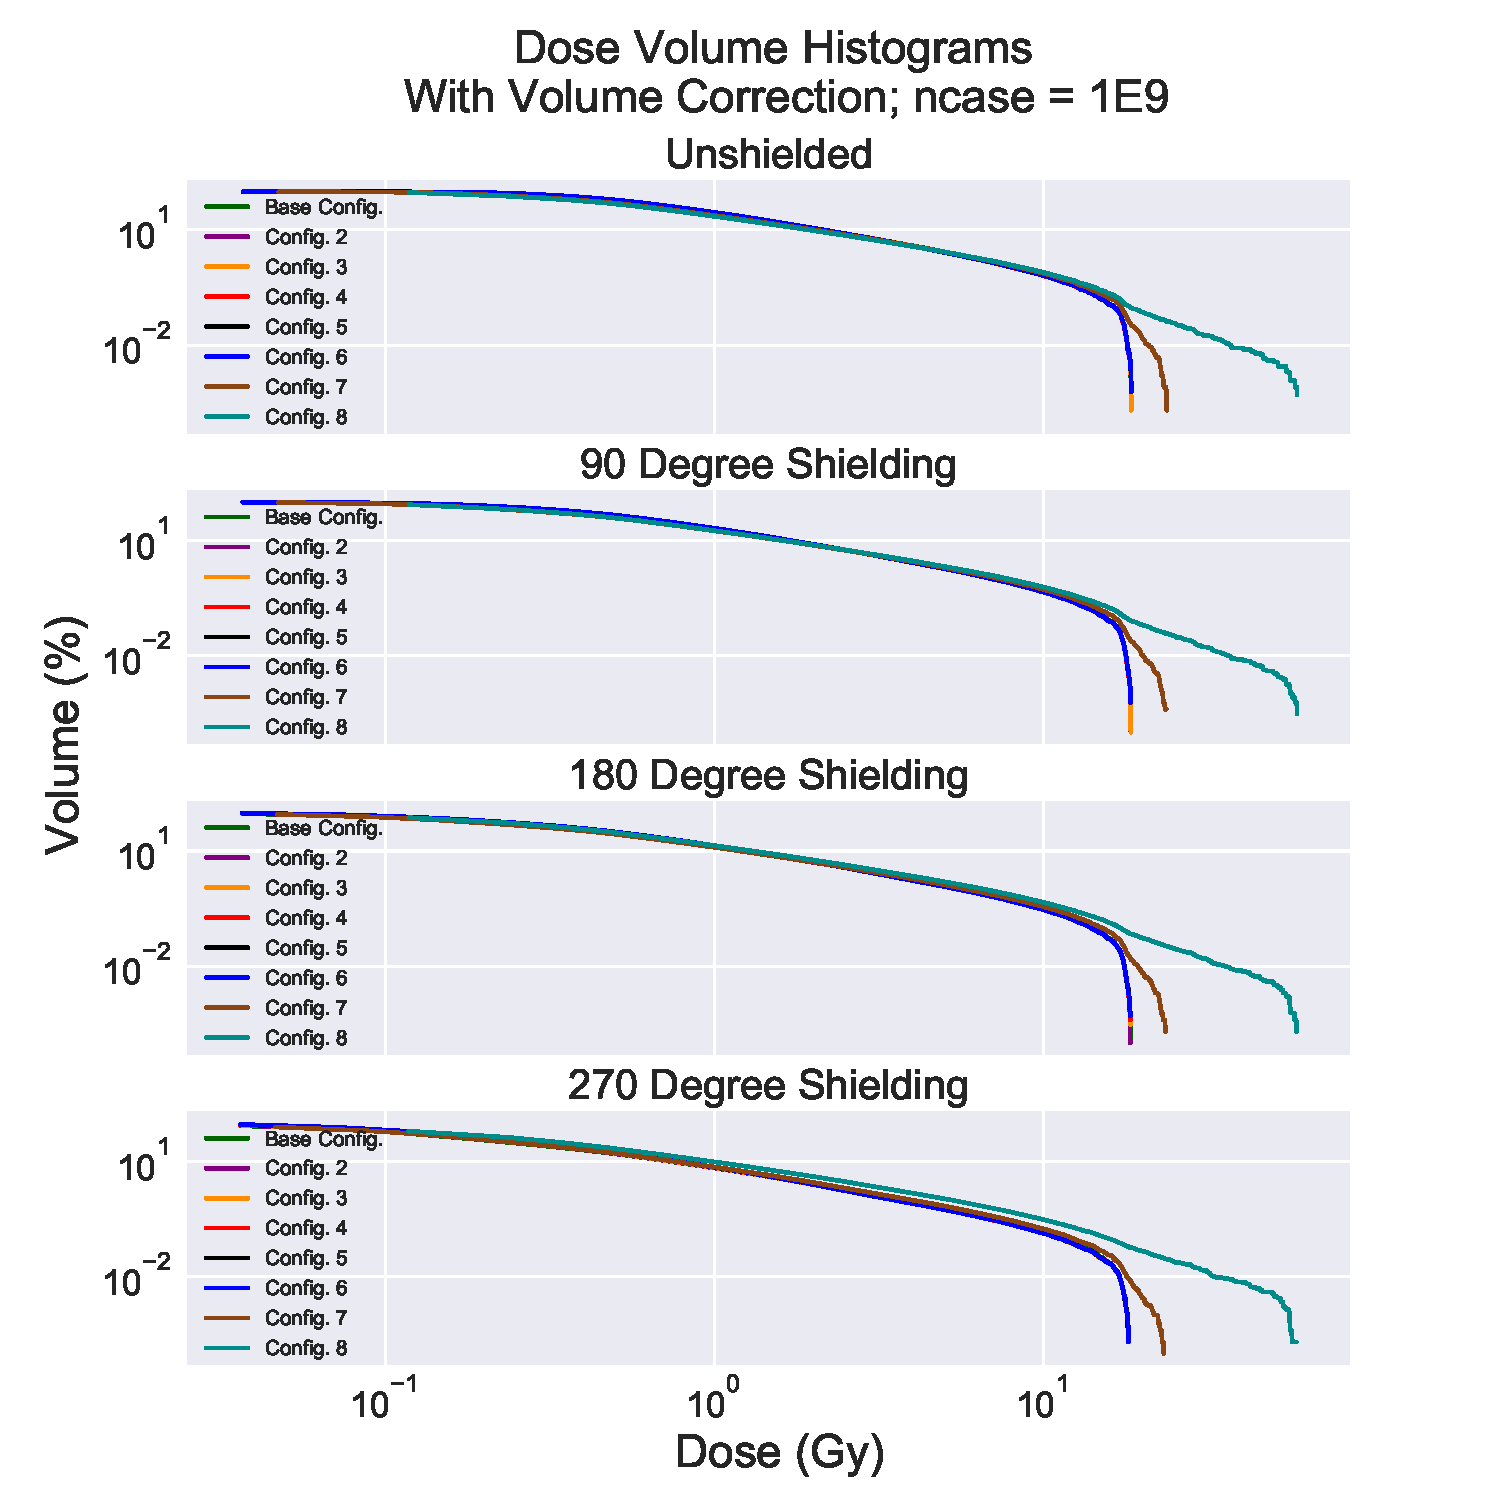
\includegraphics[scale=0.6]{cumulative_dose_volume_histogram}
	\caption{Cumulative Dose Volume Histograms.}
\end{figure}

\end{document}